\documentclass{report}
\usepackage[a4paper, left=3cm, right=3cm, top=2cm, bottom=2cm]{geometry}
\usepackage{graphicx} % Required for inserting images
\usepackage{float}
\usepackage{amsmath}
\usepackage{hyperref}

\usepackage{amsmath}
\newcommand{\Mod}[1]{\ (\mathrm{mod}\ #1)}

\title{Stochastik WS23}
\author{Meiers Thierry}
\date{November 2023}

\begin{document}

\maketitle

\chapter*{Grundlegendes} 

\subsection*{Kombinatorische Formeln}

\subsubsection{Ohne Wiederholungen}
$x = (x_1, ..., x_n)$ Vektor mit verschiedenen Einträgen.
\begin{enumerate}
    \item Es gibt $n!:=n\cdot(n-1)\cdot...\cdot1$ verschiedene Vektoren der Länge n, die dieselben Einträge wie x haben.
    \item Zieht man k-mal ohne Zurücklegen, so gibt es genau $\frac{n!}{(n-k)!}$ mögliche Ausgänge, wenn man die Reihenfolge der gezogenen Einträge beachtet.
    \item Betrachtet man die Reihenfolge nicht, so gibt es genau $\binom{n}{k}=\frac{n!}{k!\cdot(n-k)!}$ mögliche Ausgänge.
\end{enumerate}

\subsubsection{Mit Wiederholungen}
$x = (x_1, ..., x_n)$ Vektor.
\begin{enumerate}
    \item Sind genau r Einträge verschieden mit Häufigkeit $k_1, ..., k_r$, so gibt es genau $\frac{n!}{k_1!\cdot...\cdot k_r}$ verschiedene Möglichkeiten, die Einträge in einer Reihenfolge zu bringen.
    \item Sind alle Einträge verschieden, und zieht man k-mal mit Zurücklegen, so gibt es genau $n^k$ mögliche Ausgänge, wenn man die Reihenfolge betrachtet. 
    \item Betrachtet man die Reihenfolge nicht, so gibt es genau $\binom{n+k-1}{k}=\frac{(n+k-1)!}{k!\cdot(n-1)!}$ mögliche Ausgänge.
\end{enumerate}

\subsubsection*{Stirling-Formel}
Wie groß ist eigentlich n! ?
\[\displaystyle \lim_{n \to \infty} \frac{n!}{\binom{n}{e}^n \sqrt{2\pi n}} = 1 \Rightarrow n! \approx \binom{n}{e}^n \sqrt{2\pi n}\]
Bew:
\[log(n!) = \sum_{i=1}^n log(i) = \int_{1}^{n} log(x)dx + O(log(n)) = x log(x) - x + O(log(n)) = n log(n) - n + O(log(n)) \]
\[n! = e^{log(n!)} = e^{nlog(n)-n}O(n) = O(n)\binom{n}{e}^n\]

\section*{Wahrscheinlichkeitsräume und Zufalls-Variablen}

\subsection*{Zufallsvariablen}
Sei E eine Menge. Ein zufälliges Element X von E heißt (E-Wertige) Zufalls-variable. Hierbei bedeutet zufällig, dass man X eine Verteilung zuordnen kann.

\subsubsection{Verteilung einer Zufallsvariable}
\begin{itemize}
    \item Falls E ist höchstens abzählbar, so heißt X diskret und $x \rightarrow P(X=x) $ \textbf{Zähldichte} der Verteilung von X.
    \item Falls $E \subseteq R$ und für $a < b$ $P(X \in (a, b)) = \int_a^b f(x)dx$ so heißt X \textbf{stetig} und f \textbf{Dichte} der (stetigen) Verteilung von X.
\end{itemize}

\subsubsection*{Wahrscheinlichkeitsverteilung}
Sei $P(E)$ die Potenzmenge von $E, P : A \subset P(E) \rightarrow [0, 1]$ eine Abbildung. 
\begin{itemize}
    \item $P(E) = 1$
    \item $\forall a \in A \rightarrow P(a^c) = 1 - P(a)$
    \item Für paarweise disjunkte $A_1, ..., A_n$ ist $P(A_1  \bigvee ... \bigvee A_n) = \sum_{n=1}^\infty p(An)$
\end{itemize}

\subsection*{Einschluss-Ausschluss-Formel}
\url{https://www.aleph1.info/?call=Puc&permalink=ema22_4_2_Z6}

\subsection*{Bild-Verteilungen}
Ist X eine E-wertige ZV und $h : E → E'$, so ist $Y := h(X)$ eine $E'$-wertige ZV und
 \[P(Y \in B) = P(X \in h^{-1}(B))\]
Die Verteilung von Y ist Bildverteilung der Verteilung von X unter h

\section*{Unabhängigkeit}
Seien $X_1, ..., X_n$ Zufallsvariablen. Falls $P(X_1 \in A_1, ..., X_v \in A_n) = P(X_1 \in A_1) \cdot ... \cdot P(X_n \in A_n)$ für alle $A_1, ..., A_n$, so heißen $X_1, ..., X_n$ unabhängig.

\chapter*{Verteilungen und deren Eigenschaften}

\section*{Zufallszahlen}
Sei $E$ endlich und $e_1 \in E$ ein Startzustand. Des weiterem sei $T : E \rightarrow W$ eine Übergangsfunktion. Dann heißt $(x_1, x_2, ...)$ mit $x_1 := e_1 \in E$ und $x_{n+1} = T(x_n), n = 1, 2, ...$ eine Folge von Pseudozufallszahlen und $(T, e_1)$ ein Pseudo-Zufallszahlengenerator. 
\subsection*{Kongruenzgenerator}
$e_1 \in E = N_0$ Gib es $a, c, m \in N$ so dass $T(x) = ax + c \mod m$ so heißt $(T, e_1)$ linearer Kongruenzgenerator. Ist $c = 0$ so heißt $(T, e_1)$ multiplikativer Kongruenzgenerator.
\subsection*{Satz von Euler}
Ist $\delta(m)$ die Anzahl der zu m teilfremden Zahlen in $\{1, ..., m - 1\}$ und sind a, m, teilerfremd, so gilt \[a^{\delta(m)} = 1 \mod m\]

\section*{Grundlegendes}

\begin{center}
    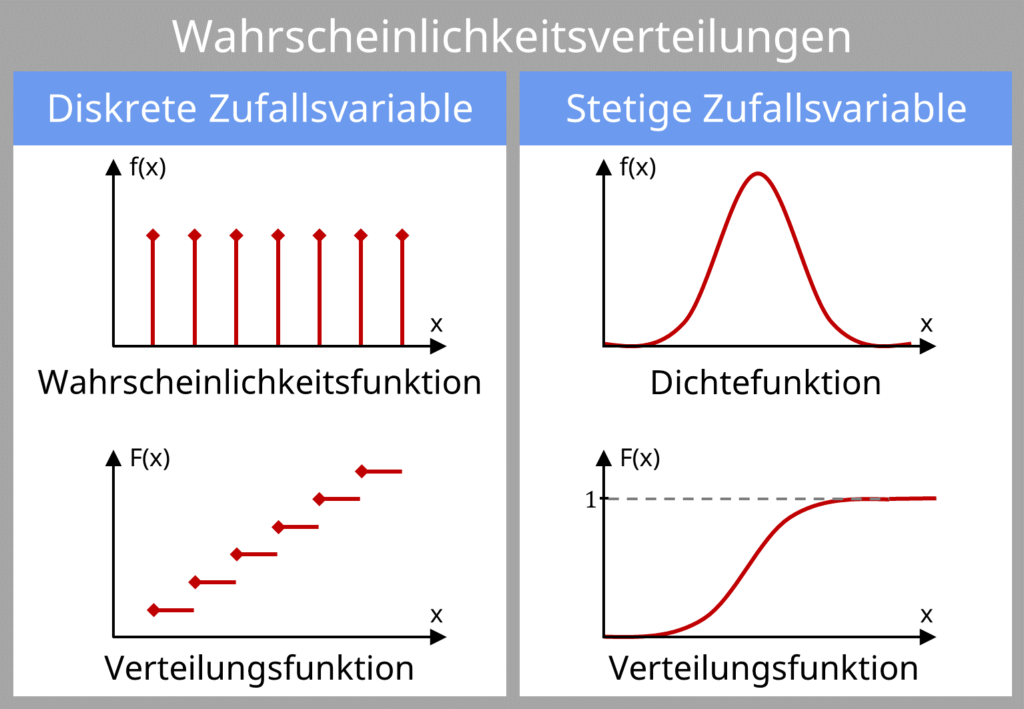
\includegraphics[width=0.5\textwidth]{media/diskretVsStetig.png}
\end{center}

\subsection*{Verteilungsfunktion}
Sei X eine $E \subseteq R$-Wertige Zufallsvariable. Dann heißt \[x \rightarrow F_x(X) := P(X \leq x)\] Verteilungsfunktion von X. Sei X reelwertige Zufallsvariable, dann gilt

\subsection*{Uniforme Verteilungen}
\subsubsection*{Diskrete}
E endlich. Ist $x \rightarrow P(X = x)$ konstant, so heißt die Verteilung von X
diskrete uniforme Verteilung und $P(X \in A) = \frac{|A|}{|E|}$
\subsubsection*{Stetige}
$E = [a, b]$ und X eine E-wertige ZV. Gilt für $[c, d] \subseteq [a, b]$ $P(X \in (c, d)) = \frac{d-c}{b-a}$ so heißt die Verteilung von X stetige uniforme Verteilung. Die Dichte ist dann $\frac{1}{b-a}dx\;\forall\;x \in [a, b]$

\subsection*{Diskrete Verteilungen ($k \in N$)}
\begin{tabular}{|l|l|l|l|}
\hline
\textbf{Verteilung} & \textbf{Formeln} & \textbf{Erwartungswert} & \textbf{Varianz} \\
\hline
Binomialverteilung $k \sim B(n, p)$ & $f(k|n,p) = \binom{n}{k} p^k (1-p)^{n-k}$ & $np$ & $np(1-p)$ \\
Poisson-Verteilung & $f(k|\lambda) = \frac{e^{-\lambda} \lambda^k}{k!}$ & $\lambda$ & $\lambda$ \\
Geometrische Verteilung & $f(k|p) = (1-p)^{k-1} p$ & $\frac{1}{p}$ & $\frac{1-p}{p^2}$ \\
Hypergeometrische Verteilung & $f(k|N,n,K) = \frac{\binom{K}{k} \binom{N-K}{n-k}}{\binom{N}{n}}$ & $\frac{nK}{N}$ & $\frac{nK}{N} \cdot \frac{N-K}{N} \cdot \frac{N-n}{N-1}$ \\
\hline
\end{tabular}

\subsection*{Kontinuierliche Verteilungen ($x \in R$)}
\begin{tabular}{|l|l|l|l|}
\hline
\textbf{Verteilung} & \textbf{Dichtefunktion} & \textbf{Erwartungswert} & \textbf{Varianz} \\
\hline
Normalverteilung $X \sim N(\mu, \sigma^2)$ & $f(x|\mu, \sigma^2) = \frac{1}{\sigma\sqrt{2\pi}} e^{-\frac{(x - \mu)^2}{2\sigma^2}}$ & $\mu$ & $\sigma^2$ \\
Exponentialverteilung $X \sim exp(\lambda).$ & $f(x|\lambda) = \lambda e^{-\lambda x}$ & $\frac{1}{\lambda}$ & $\frac{1}{\lambda^2}$ \\
Gleichverteilung & $f(x|a,b) = \frac{1}{b-a}$ für $a \leq x \leq b$ & $\frac{a+b}{2}$ & $\frac{(b-a)^2}{12}$ \\
Gamma-Verteilung & $f(x|a,\lambda) = \frac{\lambda^a x^{a-1} e^{-\lambda x}}{\Gamma(a)}$ & $\frac{a}{\lambda}$ & $\frac{a}{\lambda^2}$ \\
\hline
\end{tabular}

\section*{Pseudo-Zufallszahlen mit beliebiger Verteilung}
\subsection*{Simulation nach einer beliebigen Verteilung}
Sei \(X\) eine reellwertige Zufallsvariable mit Verteilungsfunktion \(F\). Die Pseudoinverse von \(F\) für \(x \in [0, 1]\) wird definiert als
\[ F^{-1}(x) := \inf\{q : F(q) \geq x\}. \]

Dann ist \(F^{-1}(U)\) genauso verteilt wie \(X\), wobei \(U\) eine gleichverteilte Zufallsvariable auf \([0, 1]\) ist.

\chapter*{Kenngrößen von Zufallsvariablen}
\section*{Der Erwartungswert}
Sei X eine E-Wertige Zufallsvariable und $h:E \rightarrow R$. Ist E Diskrete so heißt $E[h(x)] := \sum_{x \in E} h(x)P(X = x)$ Erwartungswert. Ist E stetig mir Dichte f, so ist $E[h(x)] := \int h(x)f(x)dx$ Erwartungswert von h(x).
Ist speziell $E \subseteq R$ und h = id, so heißt $E[X] := \sum_{x \in E} xP(X=x), E[X]:= \int xf(x)dx$ Erwartungswert von X.
\subsection*{Transformationssatz}
Sein X eine E-Wertige diskret Zufallsvariable und $h : E \rightarrow R$. Dann gilt: \[E[h(x)] = \sum_{y \in h(E)} yP(h(x) = y)\]
\subsection*{Eigenchaften des Erwartungswertes}
\begin{itemize}
    \item {Sei $a, b \in R$ Dann gilt: \[E[aX+bY] = aE[X]+bE[Y]\]}
    \item {Gilt $X\leq Y$ so ist $E[X]\leq E[Y]$}
\end{itemize}
\section*{Varianz \& Covarianz}
Sei $X$ entweder diskret $E \subseteq R-werige$ Zufallsvariable oder eine stetige Zufallsvariable und es existiert $\mu := E[X]$. Dann ist \[\sigma^2 := Var[x] = E[(X-\sigma)^2]\]
die Varianz von X. In beiden Fällen heißt $\sigma = \sqrt{Var[X]}$ die Standardabweichung von X. 
\subsubsection*{Bemerkung:}
Für diskrete Zufallsvariablen: \[Var[X] = \sum_{x \in E}(x-\mu)^2P(X=x)\]
für stetige Mit Dichte f \[Var[X] = \int(x-\mu)^2f(x)dx\]
\subsection*{Eigenschaften der Varianz}
Sei X entweder eine diskrete, $E \subseteq R$ wertige Zufallsvariable oder eine stetige Zufallsvariable. Dann gilt: \[Var[X] = E[X^2] - E[X]^2 = E[X(X - 1)] + E[X] - E[X]^2\]
Des weiterem gilt: \[Var[\sum_{i=1}^{n} X_i] = \sum_{i=1}^{n} Var[X_i]+2 \sum_{1 \leq i < j \leq n}Cov[X_i, X_j]\]
Ist insbesondere $(X_1, ..., X_n)$ paarweise unkorreliert, so gilt \[Var[\sum_{i=1}^{n}X_i] = \sum_{i=1}^{n} Var[X_i]\]
\section*{Kovarianz und Korrelationskoeffizient}
Sei X, Y diskrete/stetige Zufallszahlen, deren Erwartungswert $\mu_X := E[X], \mu_Y := E[Y]$ sowie Varianzen $\sigma^s_X := Var[X], \sigma^2_Y := Var[Y]$ existieren.
\[Cov[X, Y] := E[(X-\mu_X)(Y-\mu_Y)]\]
Gilt $Cov[X, Y] = 0$, so heißen X, Y unkorreliert.
\[Kor[X, Y] := \frac{Cov[X, Y]}{\sigma_X \cdot \sigma_Y}\] heißt Korrelationskoeffizient.
\subsection*{Eigenschaften der Kovarianz}
\begin{itemize}
    \item $Cov[X, Y] = Cov[Y, X]$
    \item $Var[X] = Cov[X, X]$
    \item $Cov[X, Y] = E[XY] - E[X]E[Y]$
    \item $Cov[X, aY+bZ] = a \cdot Cov[X, Y] + b \cdot Cov[X, Z]$
\end{itemize}
\subsection*{Cauchy-Schwarz-Ungleichung}
\[Cov[X, Y]^2 \leq Var[X]Var[Y]\]+
\subsection*{Unabhängigkeit und Unkorreliertheit}
Seien X, Y reellwertige, unabhängige Zufallsvariablen, deren Varianz existiert. Dann sind X, Y auch unkorreliert.
\chapter*{Bedingte Wahrscheinlichkeiten}
Seien X, Y Zufallsvariable und $P(X \in A) > 0$. Dann heißt \[P(Y \in B|X \in A):= \frac{P(X \in A, Y \in B)}{P(X \in A)}\] bedingte Wahrscheinlichkeit von ${Y \in B}$, gegeben ${X \in A}$. Des weiteren sei X diskret. Die Abbildung \[P(Y \in B | X) : x \rightarrow P(Y \in B | X = x)\] heißt bedingte Verteilung von Y gegeben X. Haben $(X, Y )$ gemeinsame Dichte $f (x, y)dxdy$, so heißt \[\frac{f(x, y)dy}{\frac f(x, y)dz}\] bedingte Dichte von Y gegeben X.

\end{document}
